\def\year{2015}
%File: formatting-instruction.tex
\documentclass[letterpaper]{article}
\usepackage{aaai}
\usepackage{times}
\usepackage{helvet}
\usepackage{courier}


%%%%%%%%%%%%

\usepackage{algorithm}
\usepackage{algorithmic}

\usepackage{amsthm} %for theorem and proof
\newtheorem{lemma}{Lemma}
\newtheorem{definition}{Definition}

\usepackage{amsfonts, amsmath} %for mathbb
\usepackage{amsmath,amsfonts,amssymb,amsthm}

%\newcommand{\lessgt}{><}%TODO FOR NOW...

\usepackage{verbatim}
%\usepackage{ntheorem} % framed and list of theorems [standard,framed,thref] \listtheorems{types}		%COMMENTED BY HADI
\usepackage{color}    % color
\usepackage{mdframed} %for framing 
\definecolor{light-gray}{gray}{0.97}

\newtheorem{theorem}{Theorem}

%OLD
\newcommand{\ind}[1]{\mathbb{I}[#1]}
\newcommand{\inde}{\mathbb{I}}
\newcommand{\var}{v}
\newcommand{\eq}{\leftarrow}
\newcommand{\LB}{\mathit{LB}}
\newcommand{\UB}{\mathit{UB}}
\newcommand{\B}{\mathbb{B}}
\newcommand{\E}{\mathbb{E}}
\newcommand{\I}{\mathbb{I}}
\newcommand{\R}{\mathbb{R}}
\newcommand{\F}{\mathbb{F}}
\renewcommand{\vec}[1]{\mathbf{#1}}

%NEW:
\newcommand{\tuple}[1] {\langle #1 \rangle}
\newcommand{\bvec}[1]{\textbf{#1}}
\newcommand{\indicator}{\mathbb{I}}%{I\!\!I}
\newcommand{\case}[2]{#2 &\text{ if } #1}%{#1 : #2}
\newcommand{\singlecase}[2]{#2 \quad \text{ if } #1}
\newcommand{\otherwise}[1]{#1 &\text{ otherwise}}
\newcommand{\pr}{p}
\newcommand{\nn}{0.16}
\newcommand{\nnn}{0.33}
\newcommand{\nnh}{0.23}
\newcommand{\dd}{\;\mathrm{d}} % d for integration variables e.g. dx

\usepackage{booktabs}
\usepackage{enumitem}
\usepackage{graphicx} 

%%%%%%%%%%%%














\frenchspacing
\setlength{\pdfpagewidth}{8.5in}
\setlength{\pdfpageheight}{11in}
\pdfinfo{
/Title (Symbolic Gibbs Sampling in Piecewise Algebraic Graphical Models with Nonlinear Determinism)
/Author (Put All Your Authors Here, Separated by Commas)}
\setcounter{secnumdepth}{0}  
 \begin{document}
% The file aaai.sty is the style file for AAAI Press 
% proceedings, working notes, and technical reports.
%
\title{Closed-form Gibbs Sampling for Graphical Models with Algebraic Constraints}
%\author{AAAI Press\\
%Association for the Advancement of Artificial Intelligence\\
%2275 East Bayshore Road, Suite 160\\
%Palo Alto, California 94303\\
%}
\maketitle


\input abstract

%%%%%%%%%%%%%%%%%%

\input intro

\section{Preliminaries}
\label{sect:background}
{\bf Graphical models.} Let $\vec{X} = \{X_1, \ldots, X_N\}$ be a set of random variables with realizations in the form 
$\vec{x} = \{x_1, \ldots, x_N\}$.\footnote{
In case there is no ambiguity, we do not distinguish between random variables and their realizations; e.g., we abbreviate $\pr(X_i = x_i)$ by $\pr(x_i)$.}
For the sake of notational consistency, 
throughout we assume $\vec{X}$ only contain continuous variables. 
%The generalization of the presented algorithms to hybrid discrete/continuous models is straightforward.
%Note that inference in presence of discrete deterministic constraints is already addressed in the literature (see e.g.\ \cite{li2013dynamic} for related work).
%Therefore, generalization of the presented framework to hybrid discrete/continuous models is straightforward.   
To cover both directed and undirected graphical models we use
\emph{factor graph} notation \cite{kschischang2001factor}
and represent a joint probability density $\pr(\vec{X})$ in a factorized form as follows: 
\begin{equation} \footnotesize
\label{e:factor-graph}
\pr(\vec{X}) \propto \prod_{\Psi_k \in \boldsymbol\Psi} \Psi_k (\vec{X}_k)
\end{equation}
where 
$\Psi_k$ are non-negative \emph{potential functions} 
of subsets $\bvec{X}_k$ of $\bvec{X}$. 
% and the normalization constant is not necessarily known.

%\subsection{Inference}
%A main inference task is to compute the \emph{posterior} joint density 
\noindent
{\bf Inference.} The inference task studied in this paper is to compute the \emph{posterior} joint density 
$\pr(\bvec{Q} \,|\, \bvec{E}=\bvec{e})$
of 
a subset $\bvec{Q}$ (\emph{query}) of $\bvec{X}$ 
conditioned on (realization $\bvec{e}$ of) 
variables  
$\bvec{E} \subset\bvec{X} \backslash \bvec{Q}$ (\emph{evidence}):
\begin{equation}\vspace{-0.5mm}\footnotesize
\label{e:inference}
\pr(\vec{Q} \,|\, \bvec{E} =\vec{e}) \propto 
\int_{-\infty}^{\infty} \!\! \cdots \int_{-\infty}^{\infty}
\!\!\! \pr(\bvec{Q}, \bvec{W} = \bvec{w}, \bvec{E}=\bvec{e} )
 \dd \bvec{w}
\end{equation}
where $\bvec{W} = \{W_1, \ldots, W_m\} := \vec{X} \backslash (\vec{Q} \cup \vec{E})$. % 

%Beyond the families of conjugate distributions, 
The integrals required in 
(\ref{e:inference}) 
are often intractable and hence we must often resort to MCMC methods
such as Gibbs sampling \cite{geman1984stochastic} --- the focus of this work.

\noindent
{\bf Gibbs sampling.}
 In this method drawing a sample for $\bvec{X}$ takes place in $N$ steps.
In the $i$-th step, $X_i$ is sampled conditioned on the last realization of the others:
$x_i \sim \pr(X_i \,|\, \bvec{x}_{-i})$. 
To perform this task, the following univariate (conditional) \emph{cumulative density function} (CDF)
is computed by (\ref{e:cdf}) and samples are taken via inverse transform sampling. 
%{\footnotesize
\begin{equation} \footnotesize
\label{e:cdf}
\text{CDF}(X_i  \,|\, \bvec{x}_{-i}) 
\propto
\int_{-\infty}^{X_i} \!\! \pr(X_i = t, \,\bvec{X}_{-i} = \bvec{x}_{-i})  \dd  t
\end{equation} 
%Gibbs sampling does not require any tuning
%and since it directly samples from the distribution.
% (rather than indirectly and through proposals).
% it has high effective sample size. <- provide citation if you say this
%However, in general, closed-form computation of the CDF integrals is not possible and approximations (such as \cite{gilks1992adaptive}) are costly.
%Considering that $N$ univariate integrals should be computed per sample, such approximate Gibbs samplers are typically slow.


%%%%%%%%%%%%%%%%%%%%%%%%%%%%%%%%%%%%%%%%%%%%%%%%%%%%%%%%%%%%%%%%%%%%

\section{Observed Constraints}\label{sect:determinism}

%\subsection{Collapsing Determinism}
To express an observed constraint $f(x_1, \ldots, x_n) = c$, we assume that
in the variable set over which the probability measure is defined, there exists 
a random variable $Z$ such that $\pr(Z=z | x_1, \ldots, x_n) = \delta[f(x_1, \ldots, x_n) - z]$.\footnote{
This is to prevent Borel-Kolmogorov paradox \cite{kolmogorov1950foundations}
that arises when conditioning is on an event with a probability that tends to zero 
without specifying the random variable it is drawn from. %(since such conditioning is not well defined.)
$\delta\big( f(\cdot) - z\big)$ should be thought of as a limit of a normal distribution centered at $f(\cdot)$ and a variance that tends to zero.
} 
%Therefore, the constraint corresponds the event $Z=c$.

In the following theorem, we use the calculus of Dirac deltas and generalize the concept of change of random variables to (not necessarily) reversible functions $f(x_1, \cdot)$.
Since in formula~(\ref{e:theorem1}) one variable is collapsed i.e.\ marginalized out we refer to it as \emph{dimension reduction}. 

\begin{theorem}[Dimension reduction] 
\label{theorem1}
Let, 
\[ 
\pr(Z\!=\!z | x_1, \ldots, x_n) = \delta \big( f(x_1, \ldots, x_n)-z \big)
\]
where $f(x_1, \ldots, x_n) = 0$ has real and simple roots for $x_1$ with a non-vanishing continuous derivative
$\partial f(x_1, \ldots, x_n) / \partial x_1$ at all those roots.
Denote the set of all roots by 
 %let the set of all real and simple roots of the deterministic constraints with respect to $x_1$ be
 $ \mathcal{X}_1 = \{ x_1 \; | \; f(x_1, \ldots, x_n) - z = 0 \} $. 
(Note that each element of $ \mathcal{X}_1 $
 is a function of the remaining variables $ x_2,\dots,x_n,z $.)
 Then:
\begin{equation}\footnotesize
\label{e:theorem1}
p(x_2, \ldots, x_n \,|\, Z=z) \propto 
\sum_{x_1^i \in \mathcal{X}_1} 
\frac{p(X_1=x_1^i, x_2, \ldots, x_n)}
{\Big|\big(\partial f(x_1, \ldots, x_n) / \partial x_1 \big)|_{x_1 \leftarrow x_1^i} \Big|}
\end{equation}
\end{theorem}
\begin{proof} 
{\footnotesize
$p(x_2, \ldots, x_n \,|\, Z=z) \propto$
\begin{multline}
\int_{-\infty}^{\infty}p(x_1, \ldots, x_n)p(Z=z \,|\, x_1, \ldots, x_n) \dd x_1 %\notag
%
\\=\int_{-\infty}^{\infty}p(x_1, \ldots, x_n)
\delta \big( f(x_1, \ldots, x_n) - z \big) \dd x_1 
\label{e:fand}
\end{multline}
}
According to \cite{gel1964generalized}
there is a unique way to define the composition of Dirac delta with 
an arbitrary function $h(x)$:
\begin{equation}
\label{e:gelfand}
\delta(h(x)) = \sum_{i} \frac{\delta(x - r_i)}{|\partial h(x)/\partial x|}
\end{equation}
where $r_i$ are all (real and simple) roots of $h(x)$ and $h(x)$ is continuous and differentiable in the root points. By (\ref{e:fand}), (\ref{e:gelfand})  and 
\emph{Tonelli's theorem}\footnote{Tonelli's theorem says that for non-negative functions, sum and integral are interchangeable.} 
$\pr(x_2, \ldots, x_n \,|\, Z = z) \propto$
\begin{equation*}%\footnotesize
\sum_{x_1^i \in \mathcal{X}_1} 
\frac{\int_{-\infty}^{\infty} p(x_1, x_2, \ldots, x_n)  \delta(x_1 - x_1^i) \dd x_1}
{\Big|\big(\partial f(x_1, \ldots, x_n) / \partial x_1 \big)|_{x_1 \leftarrow x_1^i} \Big|}
\end{equation*}
which implies (\ref{e:theorem1}).
\end{proof}
%

\begin{comment} % Important but no space.  -Scott
{\bf Reconstructing collapsed variables.}
%Even though we have eliminated variables, we can still generate samples for them given the sample values of the non-eliminated variables. 
If $f(x_1, \cdot)$ is reversible (w.r.t.\ $x_1$),
given the realization (e.g.\ taken sample) of variables $x_2,$ to $x_n$, the value of the \emph{collapsed variable} $x_1$ is determined by $f^{-1}(z, \cdot)$.
If not, sample value of $x_1$ is $x_1^i \in \mathcal{X_1}$ with a probability proportional to: 
$\big(
\pr(x_1^i, x_2, \ldots, x_n)  \delta(x_1 - x_1^i) \dd x_1
\big)/
{\big|\big(\partial f(x_1, \ldots, x_n) / \partial x_1 \big)|_{x_1 \leftarrow x_1^i} \big|}
$.
If more than one deterministic relationship exists, 
theorem~\ref{theorem1} can be used multiple times and the collapsed variables are reconstructed in the reverse order they are eliminated.
\end{comment}

To clarify the theorem, it is used to compute the collision model posterior $\pr(M_2, V_1, V_2 \,|\, P_\text{tot} = 3)$ as follows:

\emph{
\noindent
In this model the prior joint density ${\pr(M_1, M_2, V_1, V_2)}$ is the product of potentials in equations~(\ref{sym:u12}) and (\ref{sym:u34}) which is,
$$
\begin{cases}
\frac{1}{16 V_1 + 32} &{\text{if }\scriptstyle 0.1<M_1<2.1, \, 0.1<M_2<2.1,}
							 {\scriptstyle -2<V_1<2, \, -2<V_2 < V_1}\\
 \otherwise{0}
 \end{cases}
$$  
To apply Theorem 1, we solve {\footnotesize$(M_1 V_1 + M_2 V_2 - 3)$}
w.r.t.\ a variable (say $M_1$ with the unique solution {\footnotesize$(3 - M_2 V_2)/V_1$}).
Since,  
{\footnotesize
$$\left| \frac{\partial (M_1 V_1 + M_2 V_2)}{\partial M_1} \right| = |V_1|
$$
}
by (\ref{e:theorem1}),
$\pr(M_2, V_1, V_2 \,|\, P_\text{tot} = 3)$ is proportional to
{\footnotesize
\begin{equation}\label{e:big}  
\begin{cases}
\frac{1}{V_1(16 V_1 + 32)} &{\text{if }\scriptstyle 0<V_1, \, 0.1<\frac{3-M_2 V_2}{V_1}<2.1,}\\
							 &{\scriptstyle 0.1<M_2<2.1, -2<V_1<2, \, -2<V_2 < V_1}\\
\frac{-1}{V_1(16 V_1 + 32)} &{\text{if }\scriptstyle V_1<0, \, 0.1<\frac{3-M_2 V_2}{V_1}<2.1,}\\
							 &{\scriptstyle 0.1<M_2<2.1, -2<V_1<2, \, -2<V_2 < V_1}\\
 \otherwise{0}
 \end{cases}
%=
%\begin{cases}
%\frac{1}{V_1(16 V_1 + 32)} &{\text{if }\scriptstyle 0<V_1, \, 0.1V_1<3-M_2 V_2<2.1V_1,}\\
%							 &{\scriptstyle 0.1<M_2<2.1, -2<V_1<2, \, -2<V_2 < V_1}\\
%\frac{-1}{V_1(16 V_1 + 32)} &{\text{if }\scriptstyle V_1<0, \, 2.1V_1<3-M_2 V_2<0.1V_1,}\\
%							 &{\scriptstyle 0.1<M_2<2.1, -2<V_1<2, \, -2<V_2 < V_1}\\
 %\otherwise{0}
 %\end{cases}
\end{equation}
}
}%end emph
Using (\ref{e:big}), various queries are evaluated and depicted in Figure~\ref{fig:mom}.
These plots clearly illustrate that even in this 
low-dimensional example, collapsing of nonlinear determinism can lead
to multimodal and piecewise posteriors that do not resemble the
smooth densities often studied in the literature.  

In the next section, we introduce a class of functions which is closed under dimension reduction and consequently suitable for constraint models. 
%However, the use of PPFs as a building block for piecewise graphical models with nonlinear determinism does ensure that a large set of (non)linear deterministic relationships between random variables yield $\delta$-collapsed models
%with factors still in the PPF family.  
The only task that remains then
is to provide an automated sampling method for such models which will be presented subsequently. %in Section~\ref{sect:symbolic.gibbs}
%composed of an expressive class of PPFs, which we do in the next section.
%Reasoning on the
%family of PPFs does provide a automated solution for inference in
%presence of .  Despite the importance of the latter
%problem, it is clearly only an application of the former.
%Nonetheless, the family of PPFs and inference on them is not studied
%in the literature so far.  In the rest of the paper, we will fill this
%gap.
%%%%%%%%%%%%%%%%%%%%%%%%%%%%




%FIG BLUE1
%%%%%%%%%%%%%%%%%%%%%%%%%%%%%%%%%%%%%%%%%%%%%%%%%%%%%%%%%%%%%%%%%%%%%%%%%%
\begin{figure*}%[t!]
\vspace{-1mm}
\begin{center}
\begin{tabular}{cccccc}
   \hspace{-5mm} 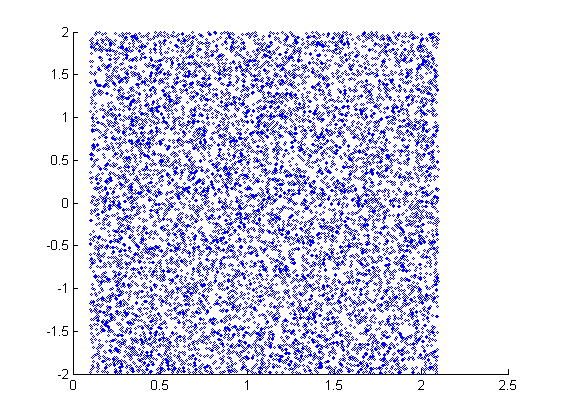
\includegraphics[width=\nn\textwidth]{Figs/col_m1_v1.png} 
& \hspace{-3mm} 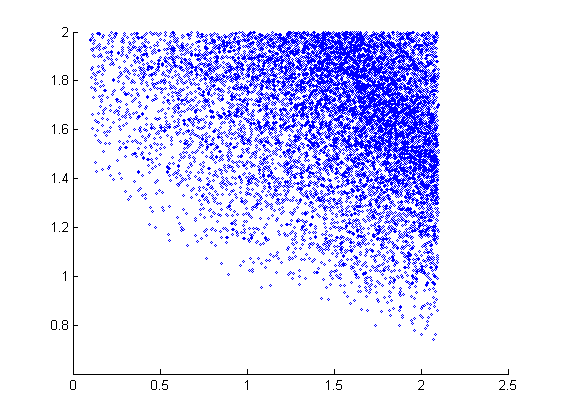
\includegraphics[width=\nn\textwidth]{Figs/col_m1v1_p3.png} 
& \hspace{-3mm} 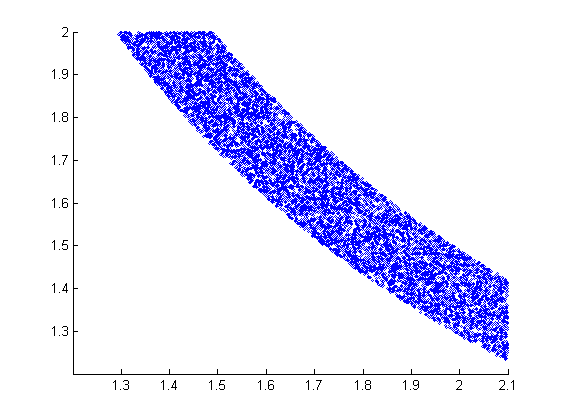
\includegraphics[width=\nn\textwidth]{Figs/col_m1v1_when_p_is_3_and_v2_is_0_dot_2.png}
& \hspace{-3mm} 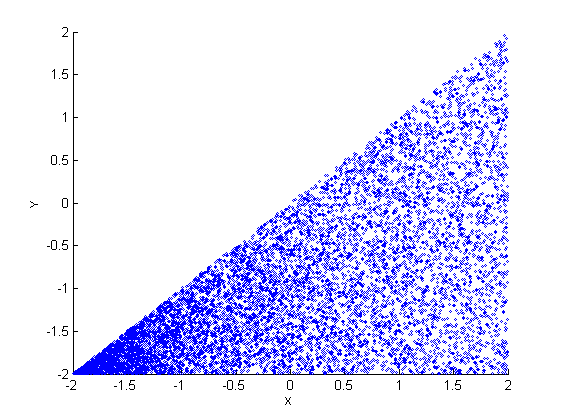
\includegraphics[width=\nn\textwidth]{Figs/col_v1v2.png}
& \hspace{-3mm} 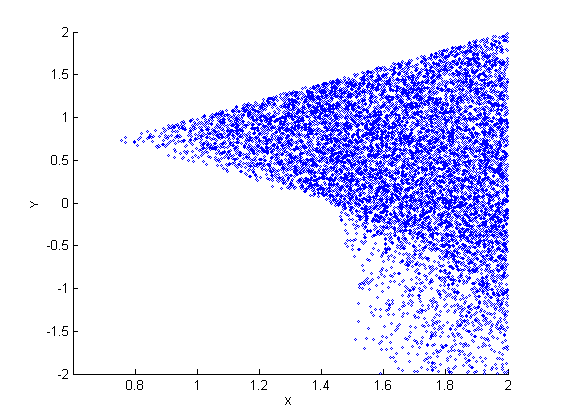
\includegraphics[width=\nn\textwidth]{Figs/col_v1v2whenPis3.png}
& \hspace{-3mm} 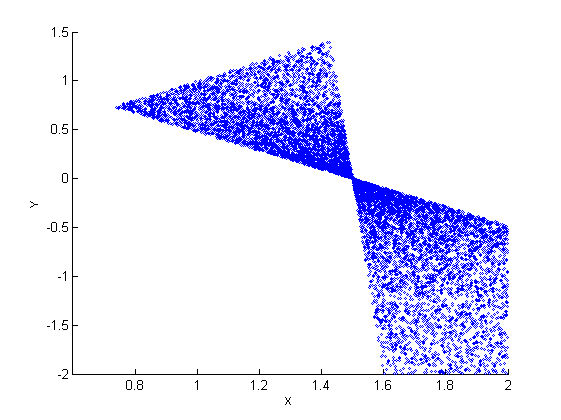
\includegraphics[width=\nn\textwidth]{Figs/colV1V2givenPis3M1is2.png}
\vspace{-1.5mm}
\\
   \hspace{-5mm} \footnotesize(a) 
& \hspace{-4mm} \footnotesize(b) 
& \hspace{-3mm} \footnotesize(c) 
&\hspace{-1mm} \footnotesize(d) 
&\hspace{-1mm} \footnotesize(e) 
&\hspace{-1mm} \footnotesize(f)\\
\multicolumn{6}{c}{}
\end{tabular}
\end{center}
\vspace{-8mm}
\caption{\footnotesize
Prior/posterior joint distributions of pairs of random variables in the \emph{collision} example. 
(a) $\pr(M_1, V_1)$,
(b) $\pr(M_1, V_1 \, | \, P_\text{tot} = 3)$,
(c) $\pr(M_1, V_1 \, | \, P_\text{tot} = 3, V_2 = 0.2)$,
(d) $\pr(V_1, V_2)$,
(e) $\pr(V_1, V_2 \, | \, P_\text{tot} = 3)$,
(f) $\pr(V_1, V_2 \, | \, M_1 =2, P_\text{tot} = 3)$
using rejection sampling on the $\delta$-collapsed model.
} 
\label{fig:mom}
\end{figure*}
%%%%%%%%%%%%%%%%%%%%%%%%%%%%%%%%%%%%%%%%%%%%%%%%%%%%%%%%%%%%%%%%%%%%%%%%%%




\section{Polynomial Piecewise Fractionals 
%Functions 
(PPFs)}
\label{sect:ppfs}
%In the introduction, it was mentioned that Gibbs sampling is the most suitable inference tool for piecewise models.
%However, Gibbs requires multiple integration per sample (see \ref{e:cdf})
% which in general cannot be performed in closed-form and in any case, is costly.
%Here, we present a class of functions that (1)~is rich enough to approximate any density, (2)~remains closed under operations required for dimension and therefore allows 

%Now that we have collapsed out determinism, we can apply Gibbs sampling. However, automated derivation of Gibbs sampling requires a univariate symbolic integral (required in (\ref{e:cdf})) which is not possible in the general case.

We introduce an expressive family of functions that is rich enough to simulate arbitrary density functions up to arbitrary precision. 
This family is the class of \emph{polynomial piecewise fractional} functions (PPFs). More formally, a PPF is a function of the form,
$f = \sum_{i=1}^m \indicator[\phi_i]\cdot f_i $ where $\indicator[\cdot]$ denotes the indicator function. Using expanded notation, 
{\footnotesize
\begin{equation}
\label{e:ppf}
f =
  \begin{cases}
  \case{\phi_1}{f_1}\\
\vdots\\
  \case{\phi_m}{f_m}    
  \end{cases}
\!\!=
  \begin{cases}
  \case{\varphi_{1,1} \lessgtr 0,\, \varphi_{1,2} \lessgtr 0,\, \ldots}{\frac{N_1}{D_1}} \\
\vdots\\
   \case{\varphi_{m,1} \lessgtr 0,\, \varphi_{m,2} \lessgtr 0,\, \ldots}{\frac{N_m}{D_m}}    
  \end{cases}
\end{equation}
}
where each \emph{sub-function} $f_i := \frac{N_i}{D_i}$ is a (multivariate) polynomial fraction and
\emph{conditions} $\phi_i$ partition the space of function variables. 
Each $\phi_i$ is a conjunction of some inequalities ($\lessgtr$ stands for  
$>$ or $<$)\footnote{
We assume the total measure on the border of partitions is 0. 
} 
where each \emph{atomic constraint} $\varphi_{i,j}$ is a polynomial.
%Evidently, this class is very expressive. Other distributions can also be approximated by this form by being \emph{Taylor series} other existing approximation tools \cite{shenoy2011inference}.

An important property of the class of PPFs is that it remains closed under operations required in (\ref{e:theorem1}). 
This paves the way for automated (and potentially multiple) implementation of Theorem~\ref{theorem1}.

By (\ref{e:mult}), PPFs are closed under elementary operations. 
{\footnotesize
\begin{align}\label{e:mult}
\begin{cases}
  \case{\phi_1}{f_1}\\
  \case{\phi_2}{f_2}    
  \end{cases}
\,
 \otimes
\,
  \begin{cases}
  \case{\psi_1}{g_1} \\
  \case{\psi_n}{g_2} 
  \end{cases}
 \, = \,
\begin{cases}
  \case{\phi_1, \psi_1}{f_1 \times g_1} \\ 
  \case{\phi_1, \psi_2}{f_1 \times g_2} \\
  \case{\phi_2, \psi_1}{f_2 \times g_1} \\
  \case{\phi_2, \psi_2}{f_2 \times g_2}
  \end{cases}
\end{align} 
\begin{align}\label{e:substitute}
f|_{x \leftarrow \frac{F}{G}}
=
\begin{cases}
  \case{{\phi_1}|_{x \leftarrow \frac{F}{G}}}{{f_1}|_{x \leftarrow \frac{F}{G}}}\\
\vdots\\
  \case{{\phi_m}|_{x \leftarrow \frac{F}{G}}}{{f_m}|_{x \leftarrow \frac{F}{G}}}    
  \end{cases}
\end{align} 
}
%
They are also closed under polynomial fractional substitution (\ref{e:substitute}). 
The reason is that in the r.h.s\ of (\ref{e:substitute}), 
(1)~sub-functions $f_i |_{x \leftarrow \frac{F}{G}}$ are polynomial fractions. 
%(which are closed under substitution).
(2)~Conditions ${\phi_i}|_{x \leftarrow \frac{F}{G}}$ are fractional but as
(\ref{e:fractional2nlpa}) shows, 
they can be restated as (multiple) case-statements with polynomial conditions. 
{\scriptsize
%\begin{tabular}{p{7cm}p{6.4cm}}
%{
\begin{equation} 
\label{e:fractional2nlpa}
\left(
 \begin{cases}
  \case{\frac{H_1}{H_2} > 0}{f_1} \\
   \vdots
 \end{cases} 
\right)
 =
{\footnotesize
\begin{cases}
  \case{H_1 > 0, H_2 > 0 }{f_1} \\ 
  \case{H_1 < 0, H_2 < 0}{f_1} \\ 
  ...
 \end{cases} 
}
\end{equation}
%}
%&{
\begin{comment}
\begin{equation}\label{e:abs}
\left|
\left(
  \begin{cases}
  \case{\phi_1}{\frac{N_1}{D_1}}\\
  \vdots
  \end{cases}
\right)
\right|
=
  \begin{cases}
  \case{N_1>0, D_1>0,\phi_1}{\frac{N_1}{D_1}} \\
\case{N_1<0, D_1<0,\phi_1}{\frac{N_1}{D_1}} \\
\case{N_1>0, D_1<0,\phi_1}{\frac{-N_1}{D_1}} \\
\case{N_1<0, D_1>0,\phi_1}{\frac{-N_1}{D_1}} \\
...
 \end{cases}
\end{equation}
\end{comment}
%}
%\end{tabular}
}
Similarly, PPFs are closed under \emph{absolute value}.%, as seen in  (\ref{e:abs}), 


\subsection{Analytic integration}
%In general, PPFs are not closed under integration; however, a 
Large subsets of PPF have closed-form single integrals. 
In the next section, we propose a sampling method that performs significantly well on such subsets. 
%As it will be seen in the next section, this leads to an extremely efficient Gibbs sampling mechanism.   
%We will show that this is also holds for a large group of PPFs.
For simplicity we only focus on the following form:

\noindent\textbf{PPF*. }
A PPF* is a PPF in which: %s as in Definition~(\ref{e:ppf}) where 
\vspace{-1mm}
\begin{enumerate}[leftmargin=2.6ex]
\item Atomic constraints $\varphi_{i,j}$
can be factorized into terms where the maximum degree of each variable is less or equal to 2. 
\item The denominator of each sub-function can be factorized into %(not necessarily distinct) 
polynomials in which the maximum degree of each variable s less or equal to 2.
\end{enumerate}
\vspace{-1mm}
% ($\text{rel-degree}(D_{i, k}) \leq 2$).%, where function $\text{rel-degree}(\cdot)$, the relative degree, is defined as follows:
 %\begin{enumerate} 
%\item Each constrain $\phi_i := \varphi_{i,1} \wedge \varphi_{i,2} \wedge \ldots$ is a conjunction of polynomial (in)equalities $\varphi_{i,j}$ such that $\text{rel-degree}(\varphi_{i,j}) \leq 4$.
%\item Each sub-function $f_i  := \frac{{N}_{i}}{{D}_{i,1} \cdot {D}_{i,2} \cdots}$
%is in the form of a fraction where the numerator ${N}_i$ 
%is an arbitrary polynomial and the denominator is factorized.
%\end{enumerate}
%\textbf{Relative degree of polynomials.} $x\text{-deg}(g)$, the degree of a polynomial $g$ w.r.t.\ a variable $x$, is the degree of $g$ if all scope variables except $x$ are considered constant. For example $x\text{-deg}(x y^2 + x^2 y z^3) = 2$. The \emph{relative degree} of $g$, $\text{rel-degree}(g)$, is:
%\[\text{rel-degree}(g) = \max_{x \in \vec{x}}(x\text{-deg}(g))\]
Here is an example of a PPF* case-statement:
{\footnotesize
\begin{equation}\vspace{-0.5mm}
{\footnotesize
\label{e:ppf*example}
\singlecase{(y^2+z^2 -1)(x^2+2xy) > 0}
{\frac{x^2 y^3 + 7xz + 10}{(5xy^2 + 2)(y + x)^3}}
}
\end{equation}
}
Note that by~\ref{e:factor-graph}, graphical models are often designed in factorized forms, therefore, the verification of PPF* conditions is often not hard. 
%The class of PPF*'s is still quite expressive. Meanwhile PPF*'s have closed form (single) integrals that are not very hard to compute automatically. 

\noindent
{\bf Analytic univariate PPF* integration.} 
Now we provide a procedure for analytic integration on PPF* functions.
It can be shown that if in a PPF* all variables except one are instantiated, 
the resulting univariate function has a closed form integral.  
This is sufficient for Gibbs sampling since in each step, only one variable is uninstantiated.
However, we want to go a step further and compute univariate integrals of multivariate piecewise functions  
\emph{without} instantiating the remaining variables to avoid the need
for an integration per sample.
%This leads to an extremely efficient implementation of exact Gibbs sampling that will be introduced in Section~\ref{sect:symbolic.gibbs}.   
This may look impossible since in the latter case, the integration bounds depend on the values of uninstantiated conditions. 
But as the following procedure shows, it is indeed possible for the PPF* class.

The following procedure computes $\int_{\alpha}^\beta f \dd x$ where $f$ is a PPF*:

\begin{enumerate}[leftmargin=2.6ex]
\item \emph{(Partitioning).}
The integral of the piecewise function $f$ is the summation of its case statement integrals:
{\footnotesize
\begin{equation*}
\int \sum_{i=1}^m \indicator[\phi_i]\cdot f_i \dd x = 
\sum_{i=1}^m \int \indicator[\phi_i] \cdot f_i \dd x
\end{equation*}
}
Therefore we only need to show that a single PPF* case-statement is integrable.

%Firstly, note that the definite integrals can be reduced to indefinite integrals:
%{
%\footnotesize\vspace{-0.5mm}
%\begin{align*}
%\int_{\alpha}^{\beta} f \dd x  = 
%\int_{-\infty}^{\infty}
%\left (
 % \begin{cases}
 % \case{x\!>\!\alpha,\, x\!<\!\beta,\, \alpha \!<\! \beta}{1}\\
% \otherwise{0}    
 % \end{cases}
%\otimes
 % f
%\right)
%\dd x
%\end{align*}
%}
\item \emph{(Canonicalization).} A PPF* case statement can be restated in the form of multiple case statements in which 
the degree of each variable in each atomic constraint is at most 2.
For instance, (\ref{e:ppf*example}) can be restated as:
\begin{equation}
\begin{cases}
\case{(y^2+z^2 -1)>0, (x^2+2xy)>0}{\frac{x^2 y^3 + 7xz + 10}{(5xy^2 + 2)(y + x)^3}}\\
\case{(y^2+z^2 -1)<0, (x^2+2xy)<0}{\frac{x^2 y^3 + 7xz + 10}{(5xy^2 + 2)(y + x)^3}}\\
\end{cases}
\end{equation}

\item \emph{(Condition solution).} For the integration variable $x$, 
a PPF* case statement can be transformed into a piecewise structure 
with atomic constraints in form $x>L_i$ or $x<U_i$ or $I_i>0$, 
where $L_i$, $U_i$ and $I_i$ are 
algebraic expressions (not necessarily polynomials) that do not involve $x$. 
%\footnote{Again, we are careless about equalities.} 
%For instance a case-statement:
%\begin{align*}
%{\footnotesize
% \begin{cases}
%  \case{(xy + z) > 0 \wedge \cdots}{f_1} \\ 
%  \vdots\\
% \end{cases} \!\!\!\!\!\!=
%\begin{cases}
%  \case{(y >0) \wedge (x>\frac{z}{y}) \wedge \cdots}{f_1} \\ 
%  \case{(y <0) \wedge (x<\frac{z}{y}) \wedge \cdots}{f_1} \\ 
 % \vdots\\
% \end{cases}
%}
%\end{align*}
%Note that in the case of quadratic constraints, these transformed cases are not necessarily polynomials.

For instance, if expressions {\footnotesize$A$}, {\footnotesize$B$} and {\footnotesize$C$} do not involve $x$,
the case statement (\ref{e:single-example})
%For instance for variable $x$, the case-statement (\ref{e:single-example})
is replaced by cases statements (\ref{e:quadratic-trans}).
\begin{equation}\footnotesize
\label{e:single-example}
\singlecase{(A \cdot x^2 + B \cdot x + C)>0}{f_1}
%\singlecase{(x^2 y + 7x^2 + x + y > 0)}{f_1}
\end{equation}
{\footnotesize
\begin{align}
\label{e:quadratic-trans}
\begin{cases}
  \case{(A>0), \, (x> \frac{-B + \sqrt{B^2 - 4 A C}}{2 A}) }{f_1} \\ 
  \case{(A>0), \, (x< \frac{-B - \sqrt{B^2 - 4 A C}}{2 A}) }{f_1} \\ 
  \case{(A<0), \, (x> \frac{-B - \sqrt{B^2 - 4 A C}}{2 A}),
                              (x< \frac{-B + \sqrt{B^2 - 4 A C}}{2 A})}{f_1}
 \end{cases}
\end{align}
}
\emph{3. (Bounding).} The bounded integral of a case statement 
associated with $\{L_i\}_i$, $\{U_i\}_i$ and $\{I_i\}_i$ 
is itself a case-statement with the same independent constraints,
 lower bound LB =$\max\{\alpha, L_i\}$ and 
 upper bound UB =$ \min\{\beta, U_i\}$.
For example:
{\footnotesize 
\begin{align*}
%\footnotesize
&\int_{\alpha}^{\beta}\!\! \Big[
\singlecase{(x>{\bf\color{blue}3}), (x>{\bf\color{blue}y}), 
(x<{\bf\color{green}y^2\!-\!7}),  ({\bf\color{red}y>0})}
{x^3 + xy} \Big] \dd x \\
%
&=\singlecase{({\bf\color{red}y>0})}
{\Big[ \int_{\max\{\alpha, \,{\bf {\color{blue}3}, \, {\color{blue}y}}\}}^{\min\{\beta, \, {\bf\color{green} y^2 - 7}\}} \!\! x^3 + xy \dd x \Big]} 
\end{align*}  
}
\emph{4. (sub-function integration).} %What remains is to compute the indefinite integrals of sub-functions. 
What is remained is to compute infinite integral of sub-functions. 
The restrictions imposed on PPF* sub-functions 
guarantee that they have closed-form %indefinite 
univariate integrals.
These integrals are computed via polynomial division 
(in case the degree of $x$ in the sub-function's numerator is more than its denominator),
followed by partial fraction decomposition.% and finally, using a short list of indefinite integration rules.

%% TODO: This barely counts as a proof... need to improve and make more complete. -Scott

%\emph{5. (aggregation).}
%The integral of the piecewise function $f$ is the summation of its case statement integrals:
%\begin{equation*}
%\int \sum_{i=1}^m \indicator[\phi_i]\cdot f_i \dd x = 
%\sum_{i=1}^m \int \indicator[\phi_i] \cdot f_i \dd x
%\end{equation*}

\end{enumerate}
%%%%%%%%%%%%%%%%%%%%%%%%%%%%%%%%%%%%%%%%%5
\section{Closed-form Gibbs Sampling}
\label{sect:symbolic.gibbs}

%Gibbs sampling is an attractive MCMC tool in the sense that it does not require known bounds or any kind of tuning.In Gibbs, drawing a sample for $\bvec{X} := (X_1, \ldots, X_N)$ takes place in $N$ steps. In the $i$-th step, $X_i$ is sampled conditioned on the current realization of the others variables:
%$x_i \sim \pr(X_i \,|\, \bvec{x}_{-i})$\cite{bishop2006pattern}.To do so, the univariate (conditional) \emph{cumulative distribution function} (CDF) is computed by (\ref{e:cdf.0}) and a sample is taken by \emph{inverse transform sampling}. 
%\begin{equation} \footnotesize
%\label{e:cdf.0}
%\text{CDF}(X_i  \,|\, \bvec{x}_{-i}) 
%\propto
%\int_{-\infty}^{X_i} \!\! \pr(X_i = t, \,\bvec{X}_{-i} = \bvec{x}_{-i})  \dd  t
%\end{equation} 
%
\emph{Closed-form Gibbs} sampling is based on a simple but significantly useful insight:
If $\pr(\bvec{X})$
has analytic integrals w.r.t.\ any variables $X_i$ (as is the case with PPF* densities),
then the costly CDF computations can be done \emph{prior to the sampling process rather than per sample}. 
It is sufficient to construct a mapping $\mathcal{F}$ from variables $X_i$ to their corresponding (unnormalized conditional) analytical CDFs. 
%then, instead of computing $N$ univariate integrals (required in Eq.~\ref{e:cdf}) per sample, we can perform the costly computations prior to the actual sampling process by constructing a map from each variable $X_i$ to its corresponding univariate symbolic CDF: 
\begin{align} \footnotesize
 \mathcal{F}\colon \{X_1, \ldots X_N\} &\to (\mathbb{R}^N \to \mathbb{R}^{+} \cup \{0\}) \notag\\
 X_i &\mapsto \int_{-\infty}^{X_i} \! \pr(X_i = t , \bvec{X}_{-i}) \dd  t 
\label{e:cdf-symbolic.0}	
\end{align}
%\begin{equation} \footnotesize
%\label{e:cdf-symbolic.0}	
%F(X_i  \,|\, \bvec{X}_{-i}) 
%\mathcal{F}(X_i) := 
%\int_{-\infty}^{X_i} \!\!\!\!\! \pr(X_i = t , \bvec{X}_{-i}) \dd  t
%\qquad \text{ for } i = 1, \ldots, N
%\end{equation} 
Note that the difference between (\ref{e:cdf}) and (\ref{e:cdf-symbolic.0}) is that in the former, 
all variables except $X_i$ are already instantiated therefore 
$\text{CDF}(X_i  \,|\, \bvec{x}_{-i})$ is a univariate function but 
$\mathcal{F}$ is $N$-variate since variables $\bvec{X}_{-i}$ are kept uninstantiated and symbolic.
%As a result, $F(X_i \,|\, \bvec{X}_{-i})$ is a multivariate analytic function. 
%as Algorithm~\ref{alg:analytic-cdf} shows, 
%we can create a map from variables $X_i$ to their corresponding closed-form CDFs.
Provided with such a map, in the actual sampling process, 
to sample $x_i \sim \pr(X_i \,|\, \bvec{x}_{-i})$,
it is sufficient to instantiate the analytical CDF associated to $X_i$ with  
$\bvec{x}_{-i}$ to obtain the appropriate univariate conditional CDF.
% Algorithm commented out.  -Scott
%(see Algorithm~\ref{alg:symbolic-gibbs}).
This reduces the number of CDF computations from $N\cdot T$ to $N$ where 
%$N$ is the dimensionality of the space of variables and 
$T$ is the number of taken samples.

If CDF inversion (required for inverse transform sampling) is also
computed analytically, then Gibbs sampling may be done fully
analytically.  However, analytical inversion of PPF*s can be very
complicated and instead in the current implementation, we approximate
the CDF$^{-1}$ computation via \emph{binary search}. 
%This requires several function evaluations per sample. Nonetheless, unlike integration, function evaluation is a very fast operation. Therefore, this suffices for highly efficient Gibbs sampling as we show experimentally in the next section.

% This algorithm is obvious and takes up space that we need. -Scott
%
\begin{comment}
%%%%%%%%%%%%%%%%%%%%%%%%%%%%%%%%%%%%%%%%%%%%%%%%%%%%%%%%%%%%%%%%%

\begin{algorithm}[hb!]%[hb!]%[tb]
\caption{{\sc SymbolicGibbs}$(\bvec{X}, \bvec{x}^{(0)}, \mathcal{F}, T)$  
\label{alg:symbolic-gibbs}}
\begin{algorithmic}
 \STATE {\bfseries Input:}
{\small random variables $\bvec{X} := \tuple{X_1, \ldots, X_N}$;
initialization 
 $\bvec{x}^{(0)} := \tuple{x_1^{(0)}, \ldots, x_N^{(0)}}$; 
a mapping $\mathcal{F}$ from $\bvec{X}$	to analytical conditional CDFs;
desired number of output samples $T$.
\STATE{\bf Output:}{ a sequence of samples.}}
{\small
%{\bf Begin}//  
\FOR{$t= 1, 2, \ldots T$}
	 \STATE $\tuple{x_1^{(t)}, \ldots, x_N^{(t)}} \leftarrow \tuple{x_1^{(t-1)}, \ldots, x_N^{(t-1)}}$    
	\FOR{ {\bf each} $X_i \in \bvec{X}$}
		\STATE $F(\bvec{X}) \leftarrow \mathcal{F}(X_i)$ \emph{\hspace*{\fill}//analytic conditional CDF w.r.t.\ $X_i$}
		%\STATE //\emph{univariate CDF w.r.t.\ $X_i$:}
		\STATE 	$\textsc{Cdf}(X_i) \leftarrow F(x_1^{(t)}, \ldots, x_{i-1}^{(t)}, X_i, x_{i+1}^{(t)}, \ldots, x_N^{(t)})$ 
        \vspace{1mm}
		\STATE //Inverse transform sampling:%\emph{$G(\infty)$ is the normalization constant}
		\STATE $u \sim \mathcal{U}(0, \text{Cdf}(\infty))$
		\STATE $x_i^{(t)} \leftarrow \textsc{Cdf}^{-1}(u)$
	\ENDFOR %end for each x_i
\ENDFOR %end for t
\STATE {\bf Return} {$\big\langle
			\tuple{x_1^{(1)}, \ldots, x_N^{(1)}}, \ldots, 
			\tuple{x_1^{(T)}, \ldots, x_N^{(T)}}
		\big\rangle$}\;
%	ForEach{}{
%	
%	}
%	\textbf{end for}\\
 %  }
   %\textbf{end for}\\   
%}
} %end small
\end{algorithmic}
\end{algorithm}
\end{comment}

%**************************************************************************
\begin{table*}[t]
\footnotesize
\caption{Parameters corresponding each experimental model}
\label{t:parameters}
\centering
\begin{tabular}{l l c l l r}
\toprule
\# &\multicolumn{1}{c}{Experiment}  &\multicolumn{1}{c}{} &\multicolumn{1}{c}{HMC} &\multicolumn{1}{c}{SMC} &\multicolumn{1}{c}{Evidence}\\
\midrule
1 & collision 		&      & $\sigma^2_{P_t} = 0.05$ & $\sigma^2_{P_t} = 0.1$ & $P_t = 1.5n$\\
2 & power line		&      & $\sigma^2_{G} = 0.02$    &$\sigma^2_{G} = 0.07$   & $G = n/10.17$ \\
\bottomrule
\end{tabular}
\end{table*}


%**************************************************************************




%FIG BLUE 2
%%%%%%%%%%%%%%%%%%%%%%%%%%%%%%%%%%%%%%%%%%%%%%%%%%%%%%%%%%%%%%%%%%%%%%%%%%
\begin{figure*}[t!]
\vspace{-1mm}
\begin{center}
\begin{tabular}{cccccc}
\hspace{-3mm}
{\footnotesize SymGibbs} 
&
{\footnotesize MH}
&
{\footnotesize HMC (high noise)}
&
{\footnotesize HMC (low noise)}
&
{\footnotesize SMC (high noise)}
&
{\footnotesize SMC (low noise)}
\\
   \hspace{-5mm} 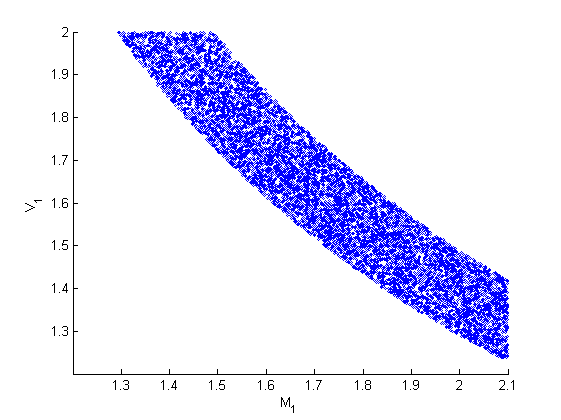
\includegraphics[width=\nn\textwidth]{Figs2/col_c_gibbs10000.png} 
& \hspace{-3mm} 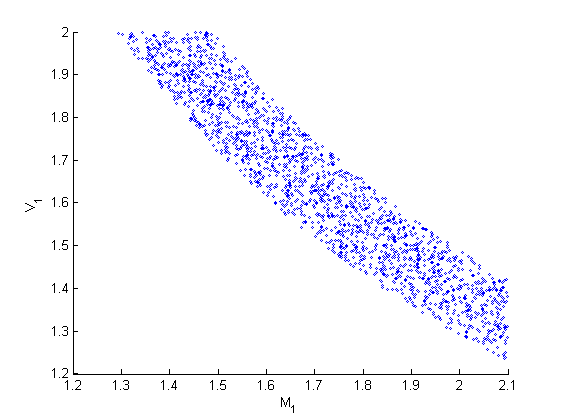
\includegraphics[width=\nn\textwidth]{Figs2/col-c-mh-10000_08.png} 
& \hspace{-3mm} 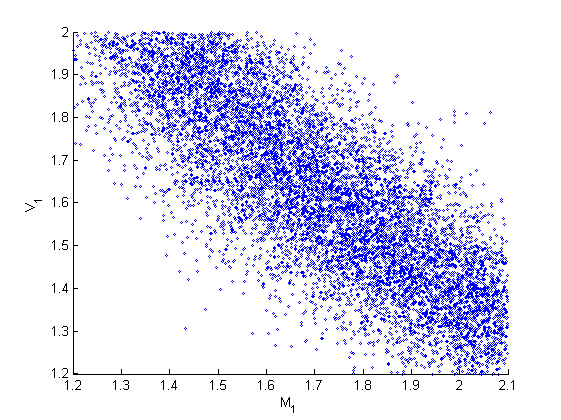
\includegraphics[width=\nn\textwidth]{Figs2/col_c_stan10000_02.png}
& \hspace{-3mm} 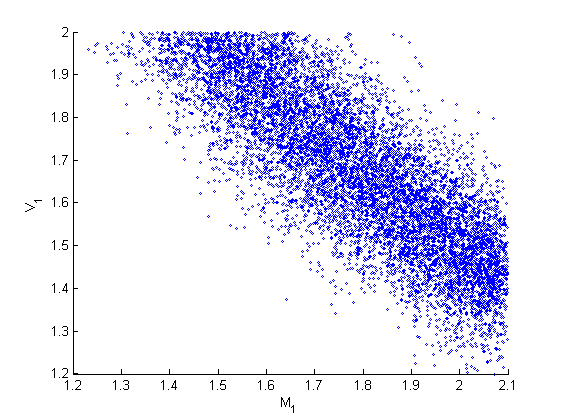
\includegraphics[width=\nn\textwidth]{Figs2/col_c_stan_10000_000001.png}
& \hspace{-3mm} 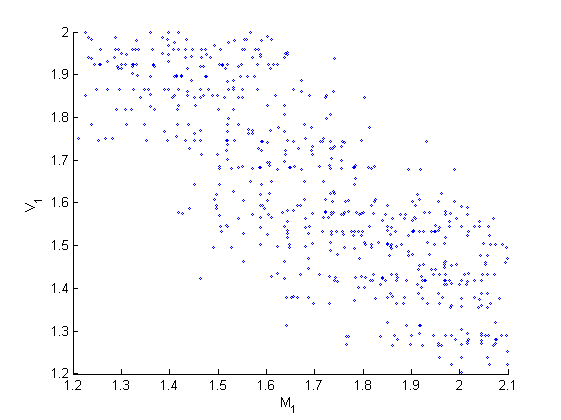
\includegraphics[width=\nn\textwidth]{Figs2/col_c_ang10000_02_001.png}
& \hspace{-3mm} 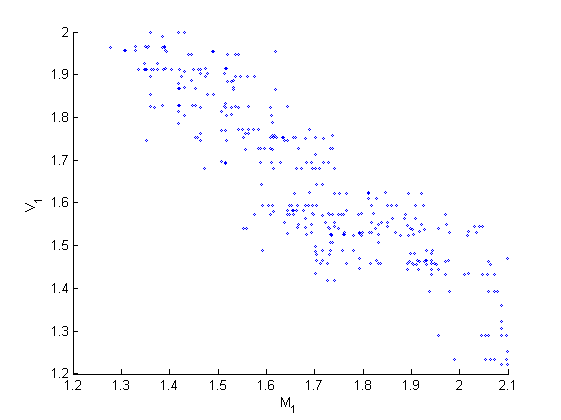
\includegraphics[width=\nn\textwidth]{Figs2/col_c_ang_10000_01_001}
\vspace{-1.5mm}
\\
   \hspace{-4mm} \footnotesize(a) 
& \hspace{-2mm} \footnotesize(b) 
& \hspace{-3mm} \footnotesize(c) 
&\hspace{-1mm} \footnotesize(d) 
&\hspace{-1mm} \footnotesize(e) 
&\hspace{-1mm} \footnotesize(f)\\
\multicolumn{6}{c}{}
\end{tabular}
\end{center}
\vspace{-8mm}
\caption{\footnotesize
10000 samples taken from the distribution Fig.~(\ref{fig:mom}-c)
using (a) \emph{Symbolic Gibbs} sampler and(b) MH with \emph{proposal variance} 0.8 
on the reduced-dimension model as well as  
(c) Hamiltonian Monte Carlo (HMC) with a measurement error variance 0.2, 
, (d) and 0.01 as well as Anglican implementation of SMC alg. with %RDB alg. with 
parameters (e)
%$V_2$ and $P_\text{tot}$ observation noise variance 
$\sigma^2_{V_2} = 0.01$, $\sigma^2_{P_\text{tot}} = 0.2$ and 
(f) $\sigma^2_{V_2} = 0.01$, $\sigma^2_{P_\text{tot}} = 0.1$
on the \emph{approximated-by-noise} model.
}
\label{fig:mom2}
\vspace{-4mm}
\end{figure*}
%%%%%%%%%%%%%%%%%%%%%%%%%%%%%%%%%%%%%%%%%%%%%%%%%%%%%%%%%%%%%%%%%%%%%%%%%%

%%%%%%%%%%%%%%%%%%%%%%%%%%%%%%%%%%%%%%%%%%%%%%%%%%%%%%%%
\section{Experimental Results}
\label{sect:experimental.results}
In this section, we are interested in (a) comparing the efficiency and accuracy of our proposed \emph{closed-form Gibbs} against other MCMC methods on  models with observed constraints as well as 
(b) studying the performance of \emph{dimension reduction} (as we propose) vs. the practice of relaxing such constraints with noise
(as often required in probabilistic programming toolkits). 
%
%The compared MCMC algorithms, the utilized measurements and the experimental models  are introduced in Sections~\ref{sect:experimental.results.algorithms}, \ref{sect:experimental.results.measures}  and \ref{sect:experimental.results.models} respectively. The experimental evaluations are discussed in  Section~\ref{sect:experimental.evaluations}.

\noindent
{\bf Algorithms compared.} 
%\label{sect:experimental.results.algorithms}
We compare the proposed \emph{closed-form symbolic Gibbs} (SymGibbs) sampler to
\emph{baseline Gibbs} (BaseGibbs) \cite{pearl1987evidential},
%i.e.\ where CDF is computed per sample, 
\emph{rejection sampling} (Rej) \cite{hammersley1964monte}, 
\emph{tuned Metropolis-Hastings} (MH) \cite{roberts1997weak}, 
\emph{Hamiltonian Monte Carlo} (HMC) using Stan probabilistic programming language  \cite{stan-manual:2014}
and \emph{Sequential Monte Carlo} (SMC) using Anglican probabilistic programming language \cite{wood2014new}.
SymGibbs and BaseGibbs require no tunings. 
MH is automatically tuned after \cite{roberts1997weak} by testing 200 equidistant proposal variances in interval 
$(0, 0.1]$ and accepting a variance for which the acceptance rate closer to 0.24.

SymGibbs, BaseGibbs and MH are run on \emph{dimension reduced} models. 
HMC on dimension reduced models produces results close to MH (not depicted for the readability of the plots). HMC and SMC with noise added to the observation are plotted. We also tested \emph{Particle-Gibbs} (PGibbs) (a variation of Particle-MCMC\cite{andrieu2010particle}) \
and \emph{random database} (RDB) (an MH-based algorithm introduced in \cite{wingate2011lightweight}) (see \cite{wood2014new}).
In our experimental models, the performance of these algorithms is very similar to (SMC) (therefore, fore readability of plots, they are not depicted). 
It should be mentioned that the state-of-the-art probabilistic programming languages, disallow deterministic relationships among continuous random variables be observed.\footnote{In BUGS \cite{lunn2009bugs}, \emph{logical nodes} cannot be given data or initial values. In PyMC \cite{patil2010pymc} deterministic variables have no \emph{observed flag}. In Stan \cite{stan-manual:2014} if you try to assign an observation value to a deterministic variable, you will encounter an error message: ``attempt to assign variable in wrong block'' while Anglican \cite{wood2014new} throws error ``invalid-observe", etc.} The solution that these off-the-shelf inference frameworks often suggest (or impose) is to approximate the observed determinism via adding noise to the observation \cite{patil2010pymc}.\footnote{
For example in the collision model, the observation $P_{\text{tot}} = 3$  would be 
approximated with a normal distribution
{\footnotesize $\mathcal{N}( P_{\text{tot}} - 3, \sigma_\eta^2)$}  
where the variance $\sigma_\eta^2$ is the noise parameter.
}
%
To soften the determinism% in HMC and SMC,
the observation of a deterministic variable $Z$ %with prior $\delta\big( G_j(\cdot) - Z_j \big)$ 
is approximated by observation of a newly introduced variable 
with a Gaussian prior centered at $Z$ and with noise variance (parameter) $\sigma^2_{Z}$. 
%instead of conditioning on a deterministic variable $X$, it is assumed that a newly introduced stochastic variable $X'$ is observed whose prior is a Gaussian centered at $X$ and with noise variance (parameter) $\sigma^2_{X}$.
Anglican's syntax requires %promotes 
adding noise to all observed variables. Therefore, in the case of SMC, stochastic observations are also associated with noise parameters.
Used parameters are summarized in Table~\ref{t:parameters}. 
SymGibbs, BaseGibbs, Rej and MH have single thread java implementations. The number of threads and other unspecified parameters of Stan and Anglican are their default settings.   
All algorithms run on a 4 core, 3.40GHz PC.% and the model compilation time of Stan and Anglican is not taken into account. 

\noindent
{\bf Measurements.}
%\label{sect:experimental.results.measures}
To have an intuitive sense of the performance of the different MCMCs,
Figure~\ref{fig:mom2} depicts 10000 samples are taken from the posterior of 
Figure~\ref{fig:mom}-c using the introduced sampling algorithms. 

For quantitative comparison,  
in each experiment, all non-observed stochastic random variables of the model  form the query vector $\bvec{Q} = [Q_1, \ldots, Q_\zeta]$.
The number of samples taken by a Markov chain $\Gamma$ up to a time $t$ is denoted by $n_{\Gamma}^t$ and  
the samples are denoted by 
$\bvec{q}_\Gamma^{(1)}, \ldots, \bvec{q}^{(n_{\Gamma}^t)}_\Gamma$
where $\bvec{q}_\Gamma^{(i)} := 
[q_{1, \Gamma}^{(i)} , \ldots, q_{\zeta, \Gamma}^{(i)}]$

%{\bf 1. Mean absolute error vs time.}
%The main measurement 
%is to compute the \emph{mean absolute error} (MAE) 
We measure mean absolute error (MAE) (equation~\ref{e:error.vs.time.measure}) vs (wall-clock) time $t$ where 
$\bvec{q}^* := [q_1^*, \ldots q_\zeta^*]$ 
is the ground truth mean query vector (that is computed manually due to the symmetry of the chosen models).
\begin{equation}\footnotesize
\label{e:error.vs.time.measure}
\textsc{MAE}_{\Gamma}(t) := \frac{1}{\zeta \cdot n_\Gamma^t} 
\sum_{j=1}^{\zeta}
\sum_{i=1}^{n_\Gamma^t}
\left|{q}^{(i)}_{j, \Gamma} - {q}_j^* \right|
\end{equation}


In each experiment and for each algorithm, $\gamma = 15$ Markov chains are run,  and for each time point $t$,
average and standard error of %mean absolute errors 
$\textsc{MAE}_{1}(t)$ to $\textsc{MAE}_{\gamma}(t)$
are plotted. 

\subsection{Experimental models}
\label{sect:experimental.results.models}

%Ex 2;  Fig 1
%%%%%%%%%%%%%%%%%%%%%%%%%%%%%%%%%%%%%%%%%%%%%%%%%%%%%%%%%%%%%%%%%%%%%%%%%%
\begin{figure*}[t!]
\vspace{-0mm}
\begin{center}
\begin{tabular}{cc}
   \hspace{-5mm} 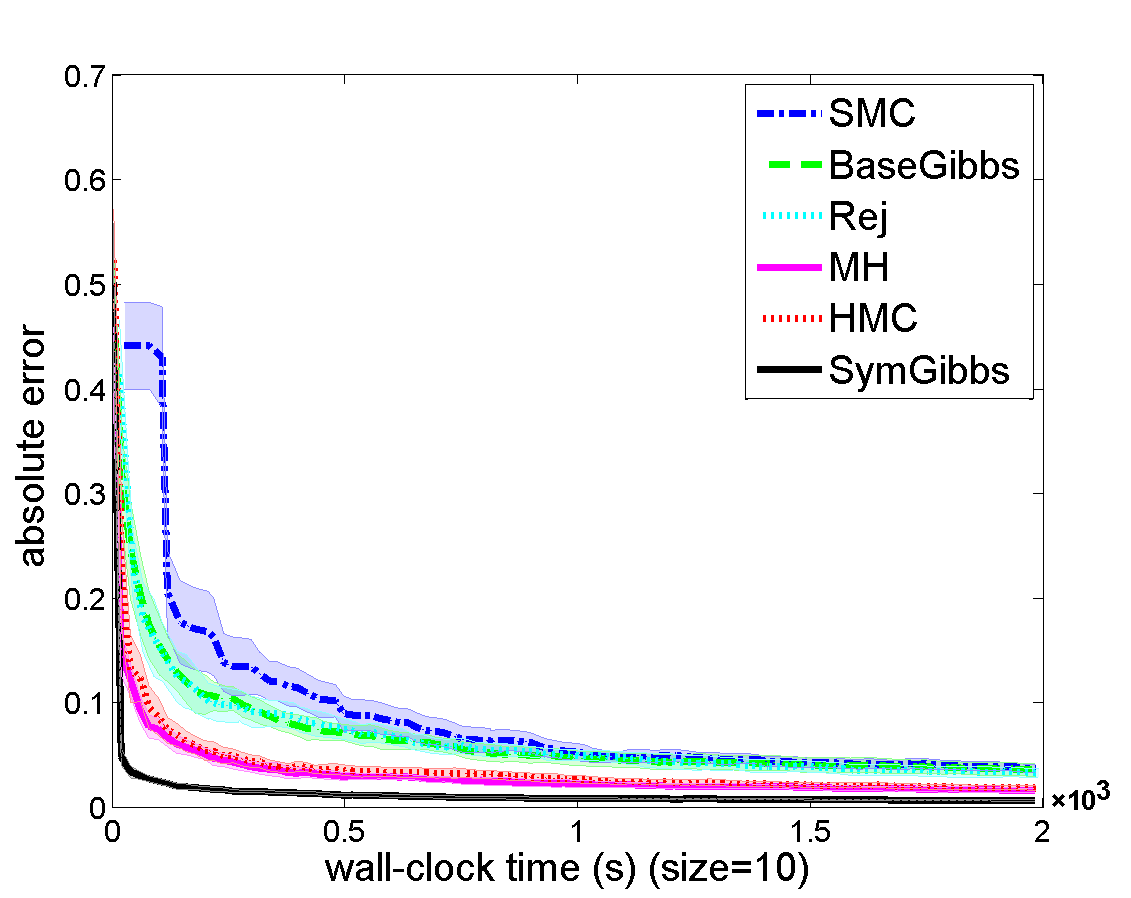
\includegraphics[width=\nnn\textwidth, height=\nnh\textwidth]{plotsx/collisionx/err-vs-time__param5-shaded.pdf} 
& \hspace{-3mm} 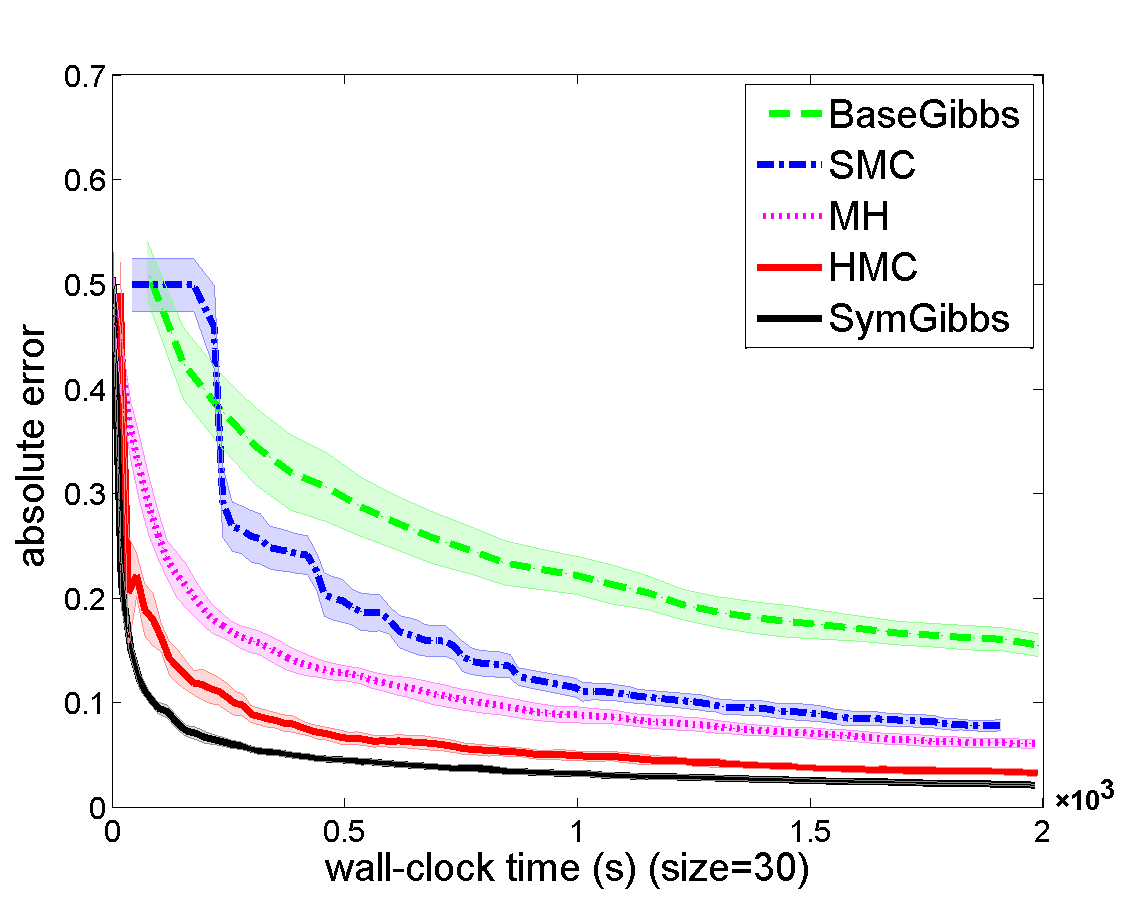
\includegraphics[width=\nnn\textwidth, height=\nnh\textwidth]{plotsx/collisionx/err-vs-time__param15-shaded.pdf} 
\vspace{-1.5mm}
\\
\hspace{-5mm} \footnotesize(a) 
& \hspace{-4mm} \footnotesize(b) 
\\
\multicolumn{2}{c}{}
\end{tabular}
\end{center}
\vspace{-6mm}
\caption{\footnotesize 
MCMC Convergence measurements in the symmetric multi-object collision model: 
Absolute error vs time for collision of (a) 4 and (b) 20 objects.}
\label{fig:multi-object.mom}
\vspace{-2mm}
\end{figure*}
%%%%%%%%%%%%%%%%%%%%%%%%%%%%%%%%%%%%%%%%%%%%%%%%%%%%%%%%%%%%%%%%%%%%%%%%%%


%Ex 2;  Fig 1
%%%%%%%%%%%%%%%%%%%%%%%%%%%%%%%%%%%%%%%%%%%%%%%%%%%%%%%%%%%%%%%%%%%%%%%%%%
\begin{figure*}[t!]
\vspace{-0mm}
\begin{center}
\begin{tabular}{cc}
   \hspace{-5mm} 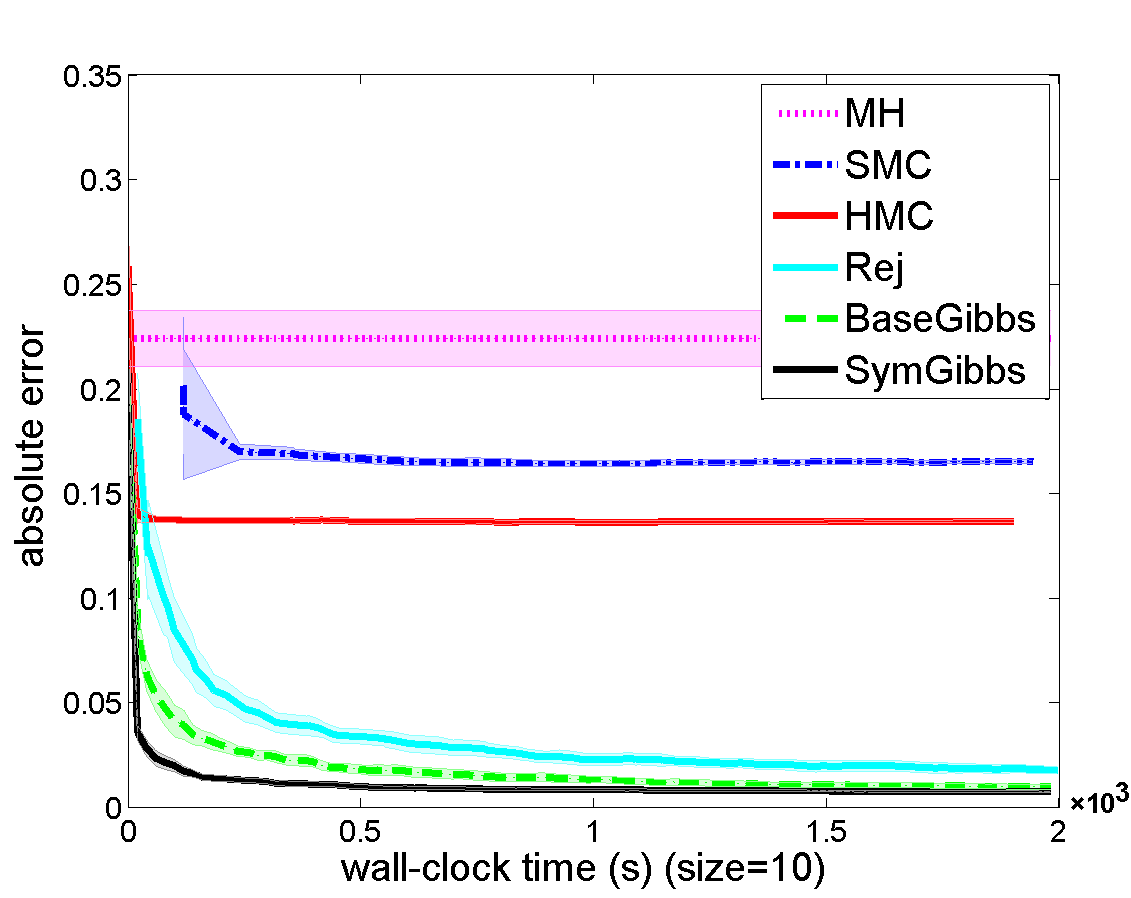
\includegraphics[width=\nnn\textwidth, height=\nnh\textwidth]{plotsx/conductancex/err-vs-time__param10-shaded.pdf} 
& \hspace{-3mm} 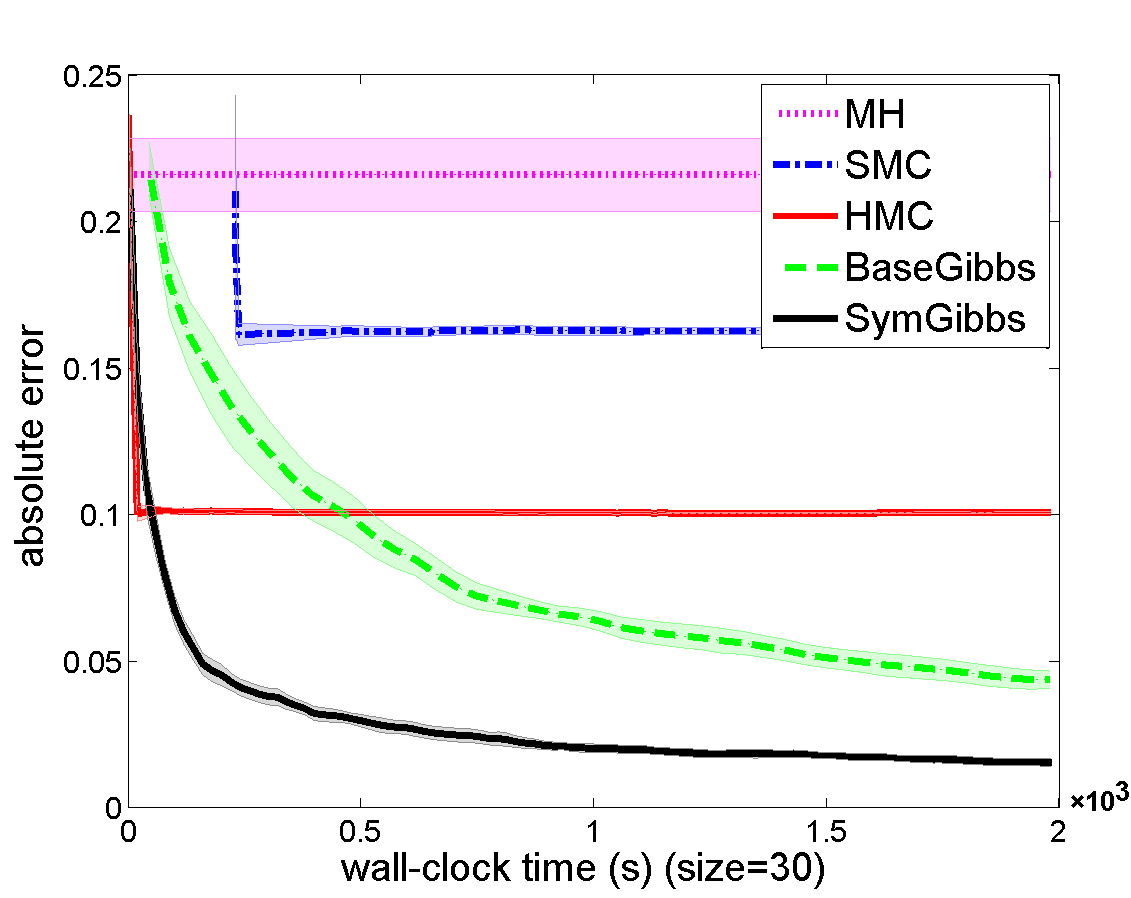
\includegraphics[width=\nnn\textwidth, height=\nnh\textwidth]{plotsx/conductancex/err-vs-time__param30-shaded.pdf} 
\vspace{-1.5mm}
\\
\hspace{-5mm} \footnotesize(a) 
& \hspace{-4mm} \footnotesize(b) 
\\
\multicolumn{2}{c}{}
\end{tabular}
\end{center}
\vspace{-6mm}
\caption{\footnotesize 
MCMC Convergence measurements in the building wiring model: 
Absolute error vs time for a model with (a) size 4 (i.e.\ 4 paralleled resistors) and (b) size 30.}
\label{fig:resistor}
\vspace{-2mm}
\end{figure*}
%%%%%%%%%%%%%%%%%%%%%%%%%%%%%%%%%%%%%%%%%%%%%%%%%%%%%%%%%%%%%%%%%%%%%%%%%%


{\bf Multi-object collision model.}
Consider a variation of the collision model in which $n$ objects collide.  
Let all $V_i$ and $M_i$ share a same uniform prior $U(0.2, 2.2)$ and the constraint be $\sum_{i=1}^n{M_i V_i} = P_{\text{tot}}$. 
The symmetry enables us to compute the posterior ground truth means  values  manually:
\begin{equation}\footnotesize
\label{e:col.GT}
M^* = V^* = \sqrt{P_{\text{tot}} / n} %\left(\frac{P}{n}\right)^{0.5}
\end{equation}
Conditioned on $P_{\text{tot}} = 1.5 n$, all masses $M_i$ and velocities  $V_i$ are queried. 
%The tested algorithms running on the reduced-dim posterior are: Symbolic Gibbs (see Section~\ref{sect:symbolic.gibbs}), 
%baseline Gibbs (CDF computation per sample), 
%MH (Metropolis-Hastings tuned manually), 
%MH automatically tuned %to reach the acceptance rate of 0.234 
%after \cite{roberts1997weak})\footnote{\label{foot:tuning} Among 200 equidistant proposal variances in %interval $(0, 0.1]$ 
%the one is chosen for which the acceptance rate is closer to 0.24. } and rejection sampling. Among the samplers that add noise to determinism, Stan's Hamiltonian MCMC with noise (variance) parameter $\sigma_P = 0.05$ and Anglican's SMC with noise parameter $0.1$ are plotted. The noise parameters are chosen manually trying to maximize the convergence rate. Other parameters are Stan and Anglican's default setting.
%By (\ref{e:col.GT}), $a_k$, the average  of $k$-th sample vector $\bvec{s}^{(k)}$, is expected to be $\sqrt{1.5}$; therefore, as the overall sampling error measure, 
%$\mathbb{E}[|{\xi} - {\xi}^*|]$ 
%$\mathbb{E}[|\bvec{a} - \bvec{a}^*|]$ is computed where $\bvec{a}$ is the vector of $a_k$ (for $k$ ranges be the number of taken samples) and all entries of vector $\bvec{a}^*$ are 1.5.
By (\ref{e:col.GT}), all elements of the ground truth vector $\bvec{q}^*$ are $\sqrt{1.5}$.
%
MAE vs. time is depicted in Figures~\ref{fig:multi-object.mom}.a \& b for a 10-D and a 30-D model, respectively.
%Time to reach error threshold $\tau = 0.3$ is plotted in Figure~\ref{fig:multi-object.mom}.c.

\noindent
{\bf Building wiring model. } 
%The next model deals with a more complicated observed determinism.
An electrical circuit composed of $n$, $10\Omega\pm5\%$ parallel resistor elements $R_i$
(with priors $\pr(R_i) = U(9.5, \, 10.5)$).
% with bell-shaped tolerance distributions (truncated quadratics, positive in the range $[8, 12]$). The posterior tolerance distribution is computed when 
The resistors are inaccessible i.e.\ the voltage drop and the current associated with them cannot be measured directly.
Given the source voltage $V$ and the total input current $I$, the posterior distribution of the element resistances are required.
Here the deterministic constraint is:
%Here, the observation can be stated as the following deterministic constraint:
\begin{equation} \footnotesize 
\label{e:reduced.mass}
 \frac{1}{R_1} + \ldots + \frac{1}{R_n} = c
\end{equation}
where $c = \frac{I}{V}$.
Equations if the form (\ref{e:reduced.mass}) are generally referred to as \emph{reduced mass} relationships and 
have applications in the electrical, thermal, hydraulic and mechanical engineering domains.

Let the observation be $c = {3n}/{(2*10.5 + 9.5)}$.
Due to the symmetry of the problem, the posterior ground truth mean is known:
\begin{equation*}
R_i^* = \frac{n}{c} = 10.166667\qquad \text{ for } i = 1, \ldots, n
\end{equation*}
MAE vs. time for networks of 10 and 30 resistors are depicted in 
Figures~\ref{fig:resistor}.a \& b respectively.
%Time to reach error threshold $\tau = 0.045$ is plotted in Figure~\ref{fig:resistor}.c.

\noindent
{\bf Experimental evaluations.}
%\label{sect:experimental.evaluations}
Plots of Figure~\ref{fig:mom2} shows that MH and SMC suffer from low \emph{effective sample size}. 
Note that the apparent sparsity of plots~\ref{fig:mom2}-b, \ref{fig:mom2}-e \& \ref{fig:mom2}-f is due to repeated samples (rejected proposals).
%
The carried out quantitative measurements 
(Figures~\ref{fig:multi-object.mom} and \ref{fig:resistor}) 
indicate that in all experimental settings,
\emph{Closed-form Gibbs} constantly and significantly performs the best.


All quantitative measurements 
(Figures~\ref{fig:multi-object.mom} and 
\ref{fig:resistor})
indicate that hard to soft constraint conversion (via introducing measurement error) ends in poor results.
Interestingly, in the Building wiring model, even in a dimensionality as low as 10, 
the Metropolis-Hasting based algorithms (i.e.\ HM, HMC and SMC) may not converge to the (manually computed) ground truth or their convergence rate is extremely low. 
This happens regardless of the way determinism is handled. 
%A reason may be as follows: It is widely known that all Metropolis-Hasting-based algorithms are sensitive to parameter tunings.Tuning takes place internally and during the burn-in period according to some heuristics.Such heuristics may not be valid in the densities studied in this paper as they are very different from the bell-shaped unimodal distributions often studied in the literature so far.
%Since Gibbs samplers directly sample from the original distributions (rather than proposal densities) they can cope well with anomalies and as our results show, always converge to the ground truth. 

\section{Conclusion}
\label{sect:conclusion}

In this paper, we introduced an expressive class of piecewise
algebraic graphical models with nonlinear determinism using factors
specified in a rich class of polynomial piecewise fractional functions
(PPFs) using polynomial partitioning constraints.
%
%To the best of our knowledge, this is the richest class of piecewise
%functions studied in the literature of graphical models and
%probabilistic inference so far.  We showed that this family is
%expressive enough to remain closed under operations required to
%transform networks with nonlinear deterministic constraints to purely
%stochastic PPF models amenable to Gibbs sampling.
%
We showed that a large subset of PPFs have symbolic univariate
integrals, which together with collapsing of nonlinear determinism, enabled the
main contribution of this paper: a fully-automated exact Gibbs sampler
called \emph{Symbolic Gibbs}.  In \emph{Symbolic Gibbs}, all
univariate CDFs required for Gibbs sampling are computed analytically
and offline.  Hence, \emph{Symbolic
  Gibbs} saves a significant amount of computation by avoiding
per-sample computations, and shows dramatically improved performance
compared to existing samplers on complex models motivated by physics
and engineering. The combination of these novel contributions should
make probabilistic reasoning applicable to variety of new applications
that, to date, have remained beyond the tractability and accuracy
purview of existing inference methods.

\small

\bibliographystyle{alpha}
\bibliography{symGibbsUAI}

\end{document}
